\documentclass[5]{article}
\usepackage[utf8]{inputenc}
\usepackage{hyperref} 

\usepackage[T1]{fontenc}
\usepackage[polish]{babel}

\title{Laboratorium 1}
\author{Piotr Witek}
\date{10 marca 2021}

\usepackage{natbib}
\usepackage{graphicx}
\usepackage{geometry}
\usepackage{tabularx}
\usepackage{array}

\begin{document}

\newgeometry{tmargin=2cm, bmargin=2cm, lmargin=2.5cm, rmargin=2.5cm}

\maketitle

\section{Znaleźć "maszynowe epsilon", czyli najmniejszą liczbę a, taką że a+1$>$1}

Aby dodać dwie liczby w reprezentacji zmiennoprzecinkowej, należy najpierw sprowadzić je do wspólnego wykładnika, cecha obu liczb musi być równa. Zatem mantysa liczby a musi być jak najmniejsza.
Zatem w systemie o precyzji p i podstawie systemu $\beta$

\[\varepsilon = \beta ^{1-p}\]


\section{Rozważamy problem ewaluacji funkcji sin(x), m.in. propagację błędu danych wejściowych, tj. błąd wartości funkcji ze względu na zakłócenie h w argumencie x}


\subsection{Ocenić błąd bezwzględny przy ewaluacji sin(x)}

\[\Delta \sin x = \left | \sin x - \sin \left ( x\left ( 1 + \varepsilon _{0} \right ) \right ) \right |\]

\subsection{Ocenić błąd względny przy ewaluacji sin(x)}

\[\frac{\Delta \sin x}{\sin x} = \frac{\left | \sin x - \sin \left ( x\left ( 1 + \varepsilon _{0} \right ) \right ) \right |}{\sin x}\]

\subsection{Ocenić uwarunkowanie dla tego problemu}

\hspace{4mm}W ogólności:

\[cond\left ( f\left ( x \right ) \right ) = \lim _{x^{*}\rightarrow x}\frac{\left | \frac{f\left ( x \right )-f\left ( x^{*} \right )}{f\left ( x \right )} \right |}{\left | \frac{x-x^{*}}{x} \right |} = \left | \frac{x\cdot f'\left ( x \right )}{f\left ( x \right )} \right| \]


Zatem dla $f\left ( x \right )=\sin x$:

\[cond\left ( f\left ( x \right ) \right ) = \left | \frac{x\cdot \cos x}{\sin x} \right | = \left | x \cot x \right |\]


\subsection{Dla jakich wartości argumentu x problem jest bardzo czuły ?}
\vspace{5mm}

\hfil
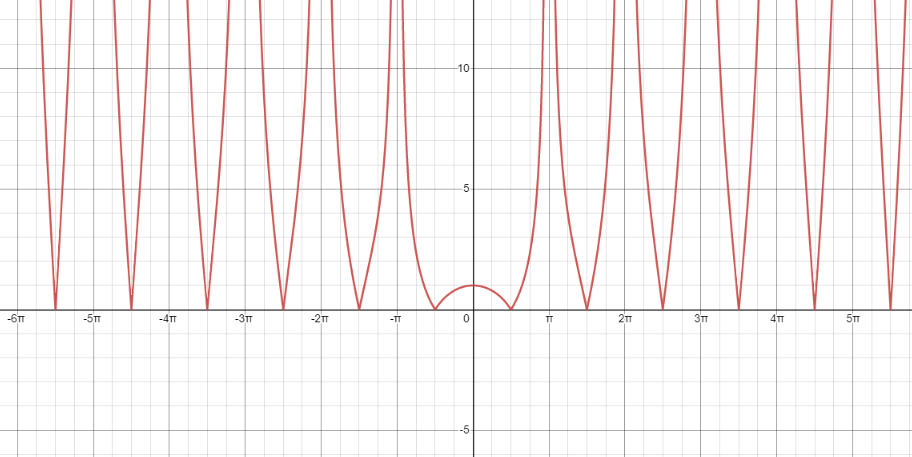
\includegraphics[scale=0.5]{wykres_lab1.PNG} \par
\vspace{3mm}
\hfil{Rysunek 1: Wykres funkcji $\left | \frac{x\cdot \cos x}{\sin x} \right | = \left | x \cot x \right | $} \par

\vspace{5mm}

Funkcja $\left | x \cot x \right |$ zmierza do $+\infty $ dla wielokrotności $\pi$ z wyjątkiem zera. Wynika z tego, że dla takich wartości argumentu x, problem jest bardzo czuły.
\vspace{3mm}

Funkcja $sin x$ jest najgorzej uwarunkowana w otoczeniu miejsc zerowych. Sama funkcja $sin x$ przyjmuje tam bardzo niewielkie wartości oraz ma największą pochodną. Najlepiej uwarunkowana jest zaś w miejscach, gdzie osiąga ekstremum (wartości funkcji -1 oraz 1). Pochodna funkcji $\sin x$ w tych punktach zeruje się.


\section{ Funkcja sinus zadana jest nieskończonym ciągiem: \\ $\sin \left ( x \right ) = x-x^{3}/3! + x^{5}/5! - x^{7}/7!+...$}


Błąd progresywny to wartość bezwględna różnicy wartości przybliżonej i rzeczywistej wartości funkcji.
\vspace{3mm}

Błędem wstecznym nazywamy moduł z różnicy wartości argumentu podstawionego do funkcji i argumentu dla którego rzeczywista wartość funkcji jest równa wartości przybliżonej.

\subsection{Jakie są błędy progresywny i wsteczny jeśli przybliżamy funkcję sinus biorąc tylko pierwszy człon rozwinięcią, tj.sin(x) ≈ x, dla x = 0.1, 0.5 i 1.0 ?}


\begin{center}
\begin{tabular}{ |c|c|c|c|c|c| } 
\hline
$x$  & $y = sin(x)$ & $\sin (x) \approx x$ & błąd progresywny & $arcsin$ & błąd wsteczny \\
\hline
0,1 & 0,099833417 & 0,1 &	0,000166583	&0,100167421	&0,000167421 \\
\hline
0,5	&0,479425539&	0,5&	0,020574461&	0,523598776&	0,023598776 \\
\hline
1&	0,841470985	&1&	0,158529015	&1,570796327&	0,570796327 \\
\hline
\end{tabular}

\\
\vspace{3mm}
{Tabela 1: Tablica błędów dla $\sin (x) \approx x$} \par
\end{center}

\subsection{Jakie są błędy progresywny i wsteczny jeśli przybliżamy funkcję sinus biorąc pierwsze dwa człony rozwinięcią, tj.sin(x) ≈ x - x^3/6, dla x = 0.1, 0.5 i 1.0 ?}



\begin{center}
\begin{tabular}{ |c|c|c|c|c|c| } 
\hline
$x$  & $y = sin(x)$ & $\sin (x) \approx x +\frac{x^{3}}{3!}$ & błąd progresywny & $arcsin$ & błąd wsteczny \\
\hline
0,1	&0,099833417 &0,099833333 &0,000000083313 &0,099999916 &0,000000083732
 \\
\hline
0,5	&0,479425539 &0,479166667 &0,000258871938 &0,499705041 &0,000294959241
 \\
\hline
1 &0,841470985 &0,833333333 &0,008137651475 &0,985110783 &0,014889216662
\\
\hline

\end{tabular}
\\
\vspace{3mm}
{Tabela 2: Tablica błędów dla $\sin (x) \approx x +\frac{x^{3}}{3!}$} \par
\end{center}

Im wieksza ilość wyrazów szeregu przybliża funkcję, tym bardziej przybliżona wartość staje się bliższa rzeczywistej, a wartości błędów stosunkowo szybko zmiejszają się. Należy nadmienić, że zgodnie z oczekiwaniami z poprzedniego zadania, w miarę zbliżania się wartości argumentów do miejsc zerowych, wartości błędów rosną. Jest to potwierdzeniem tezy, że w pobliżu miejsc zerowych funkcja $\sin x$ jest najgorzej uwarunkowana.

\section{Zakładamy że mamy znormalizowany system zmiennoprzecinkowy z $\beta = 10$, $p = 3$, $L = -98$. Jaka jest wartość poziomu UFL (underflow) dla takiego systemu? Jeśli $x=6.87\cdot 10^{-97}$ i $y = 6.81\cdot10^{-97}$, jaki jest wynik operacji $x-y$ ?}

Underflow to termin określający najmiejszą dodatnią wartość możliwą do przedstawienia w danym systemie znormalizowanym. UFL jest miarą dokładności systemu zmiennoprzecinkowego. W systemie znormalizowanym najmniejszą wartością mantysy jest 1, a najmniejsza wartość wykładnika wynosi L. Zatem:

\[UFL = \beta ^{L} = 10^{-98}\]

W ramach operacji $x-y$ otrzymamy $0.06\cdot10^{-97}=6\cdot10^{-99}$ co jest wartością mniejszą od $UFL$ zatem wynik wyniesie 0.

\section{Bibliografia}

\begin{enumerate}
  \item \url{https://pl.wikipedia.org/wiki/IEEE_754}
  \item \url{http://wazniak.mimuw.edu.pl/index.php?title=MN03}
\end{enumerate}

\end{document}
